\documentclass[11pt]{article}
\input{/Users/markwang/.preamble}
\title{CSC458 Problem Set 2}
\begin{document}

\maketitle




\section*{chapter 4}
$ $\\
\textbf{8} The telephone system uses geographical addressing. Why do you think this wasn’t adopted as a matter of course by the Internet?

\begin{solution}
    The telephone system started with stationary endpoints. Geographical location is somewhat representative of the address of endpoints, so it made sense for geographical addressing. However geographical addressing is inefficient as message routing adheres to strict geographical hierarchies. Endpoints that happened to be close to each other physically might have to go through the entire geographical hierarchy for a connection when a local network suffices to make the proper connection. Additionally, routing messages to a single region geographically is inefficient as there might be alternative best routes with less traffic.
\end{solution}

$ $\\
\textbf{9}  Suppose a small ISP X pays a larger ISP A to connect him to the rest of the Internet and also pays another ISP B to provide a fall-back connection to the Internet in the event that he loses connectivity via ISP A. If ISP X learns of a path to some prefix via ISP A, should he advertise that path to ISP B? Why or why not?


\begin{solution}
    No. Because advertising the reachability of hosts from provider ISP A to another provider ISP B implies that the customer ISP X is able to carry transit traffic. This is not a reasonable policy as such transit does not benefit ISP X but incurs cost for allowing such transit.
\end{solution}

$ $\\
\textbf{25} DHCP allows a computer to acquire a new IP address whenever it moves to a new subnet. Why is this not always enough to address the communications needs of mobile hosts?

\begin{solution}
    The problem lies in that the remote hosts are not aware of IP address changes of mobile hosts and will continue to send packets to the previous IP if no other mechanism other than DHCP exists. Conceptually, IP addresses serves 2 tasks, as identifier of an endpoint and as a way to locate the endpoint. DHCP handles locating end endpoint, but there needs to be some other rules in place for specifying identifier of mobile devices
\end{solution}

$ $\\
\textbf{26} What is the main downside of requiring traffic destined to a mobile node to be sent first to its home agent?

\begin{solution}
    It may be that route from correspondent node to mobile node may be suboptimal. An extreme example would be the correspondent node and the mobile node are in the same network but the home agent of the mobile node is located at some remote place in the internetwork. It requires that all packets be traversing the Internet to reach the home agent and then back to the mobile node. This is certainly a major drawback
\end{solution}



\section*{Chapter 5}

$ $\\
\textbf{12} Suppose TCP operates over a 1-Gbps link.

\begin{enumerate}
    \item Assuming TCP could utilize the full bandwidth continuously, how long would it take the sequence numbers to wrap around completely?
    \begin{solution}
        Time period for a 32bit sequence number to wrap around depends on how fast data can be transmitted, i.e. how fast the sequence number space can be consumed. Note each sequence number addresses 1 byte. So we have 
        \[
            4GB / 1Gbps = 8 * 4Gbits / 1Gbps = 32 s
        \]
    \end{solution}
    \item Suppose an added 32-bit timestamp field increments 1000 times during the wraparound time you found above. How long would it take for the timestamp to wrap around?
    \begin{solution}
        \[
            4 \times 10^9 / 1000 \times 32s = 1.3 \times 10^8 s
        \]
    \end{solution}
\end{enumerate}


$ $\\
\textbf{16} Suppose an idle TCP connection exists between sockets A and B. A third party has eavesdropped and knows the current sequence number at both ends.

\begin{enumerate}
    \item Suppose the third party sends A a forged packet ostensibly from B and with 100 bytes of new data. What happens? (Hint: Look up in Request for Comments 793 what TCP does when it receives an ACK that is not an “acceptable ACK.”)
    \begin{solution}
        A would send an ACK to B with an updated sequence number that takes account of the 100bytes sent by third party. However, A's ACK will be outside the B's window and so B will respond with an empty ACK segment with its own sequence number 
    \end{solution}
    \item Suppose the third party sends each end such a forged 100-byte data packet ostensibly from the other end. What happens now? What would happen if A later sent 200 bytes of data to B?
    \begin{solution}
        Both A and B will send an ACK for the forged 100-bytes data. However, both would be outside of the window and will send an emtpy ACK with their their current (updated) sequence numbers. These reciprocal ACKs' for forged data will continue to exchange between A and B since neither received the 100-bytes data \\
        If A sends 200 bytes, then B would discard the first 100 bytes because it is before the current sequence number and is regarded as duplicates and buffer the latter 100 bytes. Then B would send a proper ACK to A with the updated sequence number
    \end{solution}
\end{enumerate}


$ $\\
\textbf{32} Consult Request for Comments 793 to find out how TCP is supposed to respond if a FIN or an RST arrives with a sequence number other than NextByteExpected. Consider both when the sequence number is within the receive window and when it is not

A FIN or RST must lie in the current receive window. A RST outside this win- dow is ignored; TCP responds to an out-of-window FIN with the current ACK:


\begin{solution}
    \begin{enumerate}
        \item \textbf{out-of-window} \\
        \begin{enumerate}
            \item \textbf{FIN} not accpetable, respond with ACK reply with the sequence number, then drop the unacceptable segment
            \item \textbf{RST} not acceptable, segment is ignored
        \end{enumerate}
        \item \textbf{within receive window} \\
        \begin{enumerate}
            \item \textbf{FIN} Signal user connection closing and return any pending RECEIVEs with same message. Send acknowledgement for the FIN. Idea is that FIN gracefully closes the connection after receiving the remaining bytes
            \item \textbf{RST} The connection is closed. Any outstanding RECEIVEs and SEND receives RST responsees. all segment queues flushed. User receive unsolicited general connection reset signal. Enter CLOSED state, delete TCB. Immediate close down implies that remaining bytes are lost.
        \end{enumerate}
    \end{enumerate}
\end{solution}

$ $\\
\textbf{39} When TCP sends a $\langle SYN,SequenceNum=x \rangle$ or $\langle FIN, SequenceNum = x\rangle$, the consequent ACK has
Acknowledgment = x + 1; that is, SYNs and FINs each take up one unit in sequence number space. Is this necessary? If so, give an example of an ambiguity that would arise if the corresponding Acknowledgment were x instead of x + 1; if not, explain why.


\begin{solution}
    \begin{enumerate}
        \item \textbf{SYN} Here incrementing sequence number is not necessary since any subsequent data would also acknowledge the SYN that started the connection
        \item \textbf{FIN} Here incrementing sequence number is essential since there is no way of sender distinguishing ACK received as either acknowledgement to FIN or acknowledgement to a previous data transmission. 
    \end{enumerate}
\end{solution}

\section*{Chapter 6}

$ $\\
\textbf{4} Suppose two hosts A and B are connected via a router R.The A–R link has infinite bandwidth; the R–B link can send one packet per second. R’s queue is infinite. Load is to be measured as the number of packets per second sent from A to B. Sketch the throughput-versus-load and delay-versus-load graphs, or if a graph cannot be drawn, explain why. Would another way to measure load be more appropriate?

\begin{solution}
    Because R-B link is able to send 1 packet per second, load cannot exceed 1. Therefore both graphs' curve is undefined for load greater than 1. For delay-versus-load graph, the delay of sending packet from A to B is roughly equivalent to the bottleneck link R-B which has a constant delay of 1s for each packet for load less than or equal to 1. For throughput(power)-versus-load graph, we have 
    \[
        power = \frac{load}{delay}
    \]
    so the curve is a shows a linear relationship between load and power, with slope of 1.
    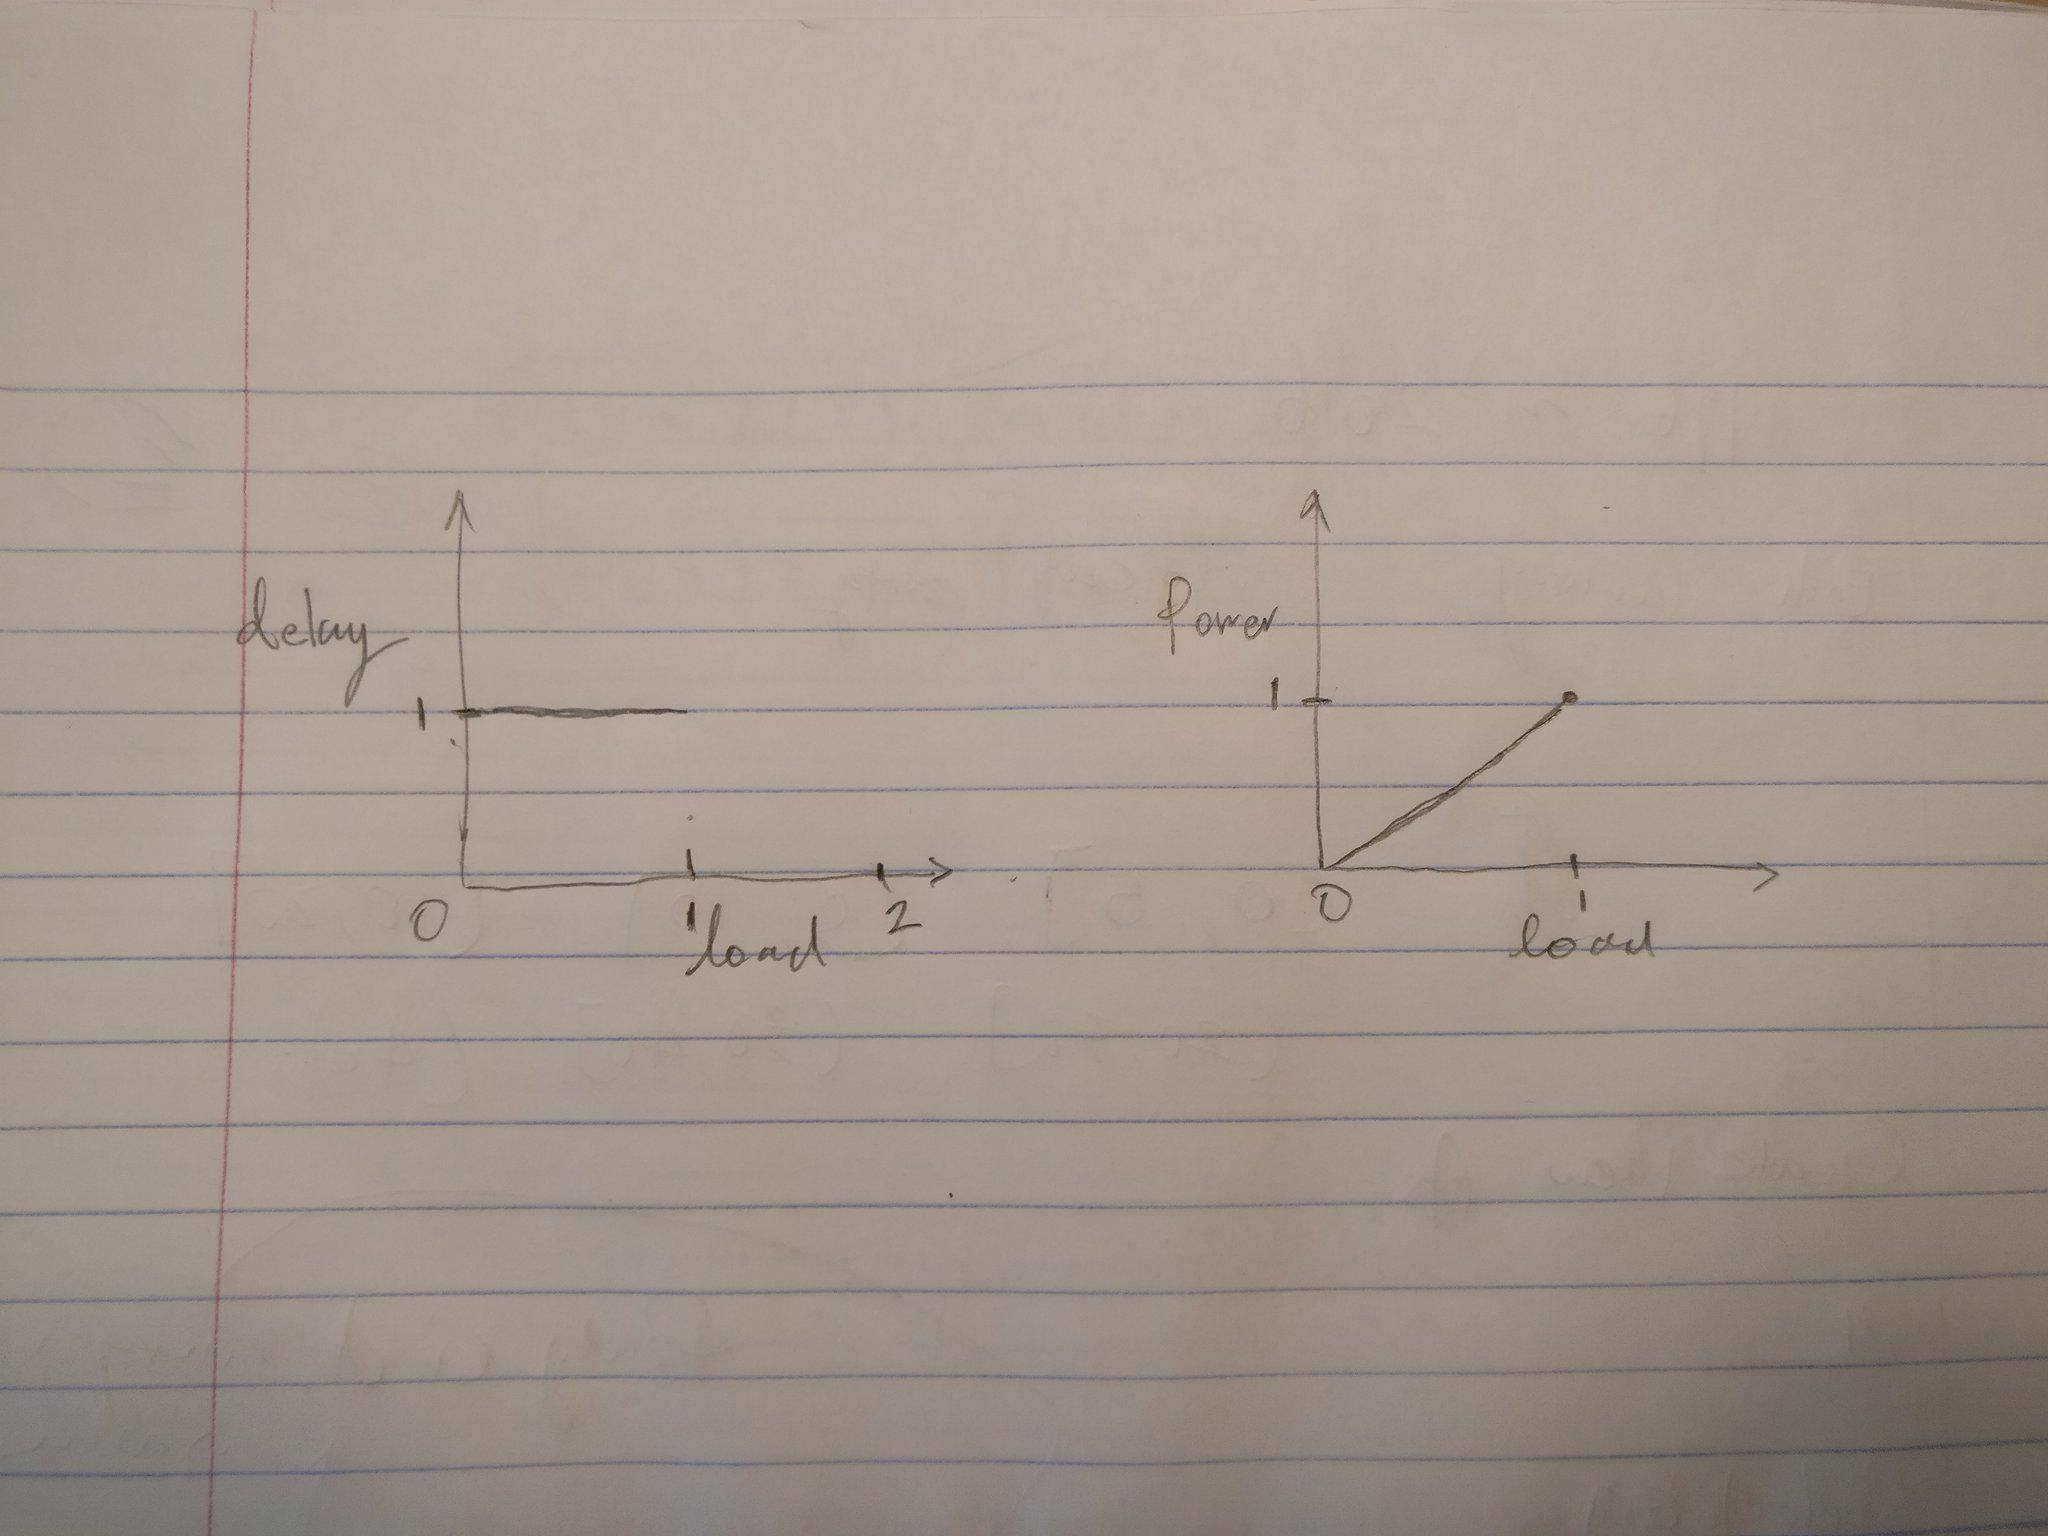
\includegraphics[width=\textwidth]{figure1.jpg}
\end{solution}



$ $\\
\textbf{7} Suppose a congestion-control scheme results in a collection of competing flows that achieve the following throughput rates: 200 KBps, 160 KBps, 110 KBps, 95 KBps, and 150 KBps.


\begin{enumerate}
    \item Calculate fairness index for this scheme
    \begin{solution}
        \[
            f = \frac{(\sum_i x_i)^2}{n \sum_i x_i^2} = \frac{715^2}{5 \times 109225} = 0.93
        \]
    \end{solution}
    \item Now add a flow with a throughput of 1000KBps to above and recalculate the fairness index 
    \[
        f = \frac{1715^2}{5\times 1109225} = 0.53
    \]
\end{enumerate}    




$ $\\
\textbf{16} Assume that TCP implements an extension that allows window sizes much larger than 64 KB. Suppose that you are using this extended TCP over a 1-Gbps link with a latency of 50 ms to transfer a 10-MB file, and the TCP receive window is 1 MB. If TCP sends 1-KB packets (assuming no congestion and no lost packets):
\begin{enumerate}
    \item How many RTTs does it take until slow start opens the send window to 1MB? 
    \begin{solution}
        Slow start doubles the congestion window size on each RTT. Starting from a window size of 1 packet, we have
        \[
            \frac{1MB}{1KB} = 2^{10}
        \]
        so after 10 RTT we get to a receive window size of 1MB
    \end{solution}
    \item How many RTTs does it take to send the file?
    \begin{solution}
        Note after $i$-th RTT, the window size is $2^i$. The size of segment transferred is a geometric series. Define $S_n$ be total size of segments transferred after $n-1$-th RTT. To find number of RTTs to send the file we find smallest $n$ such that this inequality is satisfied
        \[
            S_n = \frac{1-2^{n}}{1-2} \geq 10MB
        \]
        we have $n=14$ 
    \end{solution}
    \item If the time to send the file is given by the number of required RTTs multiplied by the link latency, what is the effective throughput for the transfer? What percentage of the link bandwidth is utilized?    
    \begin{solution}
        1 RTT is 0.1s. So 14RTT yieds a delay of 1.4s. The effective throughput is calculated as 
        \[
            throughput = \frac{10MB}{1.4s} = 7.14 MB/s
        \]
        which is 
        \[
            percent = \frac{7.14MB/s}{1Gbps} = \frac{57.1Mb}{1Bbps} = 5.7% 
        \]
        of the total link bandwidth
    \end{solution}
\end{enumerate}




$ $\\
\textbf{27} Consider the TCP trace in Figure 6.28. Identify time intervals representing slow start on startup, slow start after timeout, and linear-increase congestion avoidance. Explain what is going on from T = 0.5 to T = 1.9. The TCP version that generated this trace includes a feature absent from the TCP that generated Figure 6.11. What is this feature? This trace and the one in Figure 6.13 both lack a feature. What is it? 

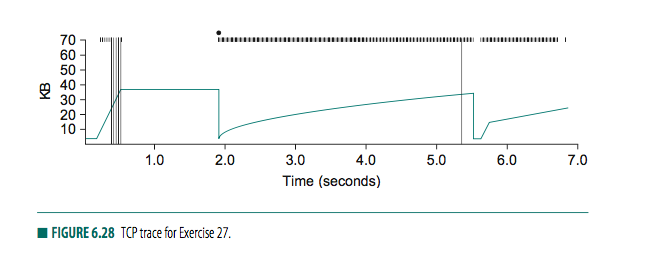
\includegraphics[width=\textwidth]{tcptrace.png}

\begin{solution}
    \begin{enumerate}
        \item slow start on startup is around time period 0 to 0.5s. 
        \item slow start after timeout is around time period 5.7s to 5.8s in response to fast retransmit of the lost packet
        \item linear-increase congestion avoidance is around time period 2s to 5.5s in response to a coarse-grained timeout
        \item From T=0.5 to T=0.9, the sender sent an entire window worth of packets and is blocked waiting for ACK reply. Therefore window size stays constant
        \item This TCP version has fast retransmission at T=5.5 while its missing from Figure 6.11
        \item This trace and Figure 6.13 both lacks fast recovery. Because in both cases, it is clear that we have fast retransmission but the congestion window size dropped to 1 instead of half of the window size
    \end{enumerate}
\end{solution}


\end{document}
